\documentclass[spanish,11pt,letterpaper]{article}

\usepackage[spanish]{babel}
\usepackage[utf8]{inputenc}
\usepackage{authblk}
\usepackage{amsmath}
\usepackage{amssymb}
\usepackage{amsthm}
\usepackage[margin=1in]{geometry}
\usepackage{graphicx}
\usepackage{hyperref}
% \usepackage{listings}
% \usepackage{xcolor}

\renewcommand{\vec}[1]{\mathbf{#1}}
\DeclareMathOperator*{\argmax}{arg\,max}
\decimalpoint

\title{{\Huge Is this Loss?}\\
Sistema de reconocimiento de objetos en imágenes}
\author{Hernández Chiapa David Felipe\\
López García Gilberto Isaac}
\affil{Facultad de Ciencias\\Universidad Nacional Autónoma de México}
\date{\small\today}

\begin{document}

\maketitle

\section{Introducción}

\section{Descripción del problema}

\section{Redes Neuronales Convolucionales}



\subsection{Capa de convolución}



\subsection{Pooling}



\subsection{Perceptrón Multicapa}



\subsection{Espacio de Hipótesis}

Las redes neuronales convolucionales para reconocimiento de objetos en imágenes
son funciones que asignan a sus entradas, imágenes de $N$ pixeles de alto por $M$
pixeles de alto, una etiqueta o categoría, las imágenes se pueden representar
como tensores de orden C, esto es, elementos del espacio
$\mathbb{R}^{N\times M\times C}$, donde $C$ es el número de canales, que puede ser
1 si se trabaja en escala de grises, 3 si se trabaja con colores (como RGB), etc.

Las entradas de estos tensores toman valores en un conjunto finito: $\{0,\ldots,255\}$,
pero dado que se requiere hacer operaciones aritméticas con sus valores de entrada
es conveniente verlos como números reales. Si tenemos entonces $K$ categorías
distintas, existe un total de $K^{256^{NMC}}$ funciones de clasificación para
imágenes, pero de la misma forma que con los árboles de decisión, existen múltiples
redes convolucionales capaces de computar la misma función.

Nuestro espacio de hipótesis son todas las redes convolucionales para clasficación
de imágenes en resolución $250 \times 250$ con 1 canal en escala de grises y 3
canales en RGB, con $K = 2$ categorías. Esto es al menos
\[ 2^{256^{250^2}} \text{  y  } 2^{256^{250^2 \cdot 3}}\]
redes convolucionales.

\subsection{Ventajas y desventajas}


\section{Propuesta e implementación}

Para la clasificación de imágenes en nuestras dos categorías \texttt{loss\_edit}
y \texttt{not\_loss}, donde la primera son edits de Loss y la segunda memes
variados, utilizaremos una red neuronal convolucional, la entrenaremos para que
aprenda a determinar qué imágenes o memes son edits de Loss, los cuales siguen
un patrón muy específico, imitando el cómic Loss%
\footnote{\url{http://cad-comic.com/comic/loss/}} (ver Figura ~\ref{fig:loss}).

Una primera aproximación sería tratar de clasificar imágenes en escala de grises
pues lo que importa para la clasificación es reconocer los objetos que aparecen
en ellas y comparar su orientación con el patrón buscado. Por desgracia existen
edits basados en la distinción de colores (ver Figura ~\ref{fig:color}), por lo
que podría ser más preciso trabajar con colores (por si distintos colores se
``funden'' en la escala de grises por tener un tono similar).

Una idea que surgió poco después fue no trabajar con las imágenes originales, sino
con las aristas. Usando el Algoritmo de Canny para extraer las aristas, es decir,
las siluetas de las formas o polígonos, se podría facilitar el trabajo de
clasificación, pero al intentar esto nos dimos cuenta que podría no ayudar o
incluso dificultar la tarea de nuestros modelos. Más adelante se hablará de los problemas
econtrados que nos llevaron a descartar esta idea en el trabajo.

\begin{figure}[h]
\centering
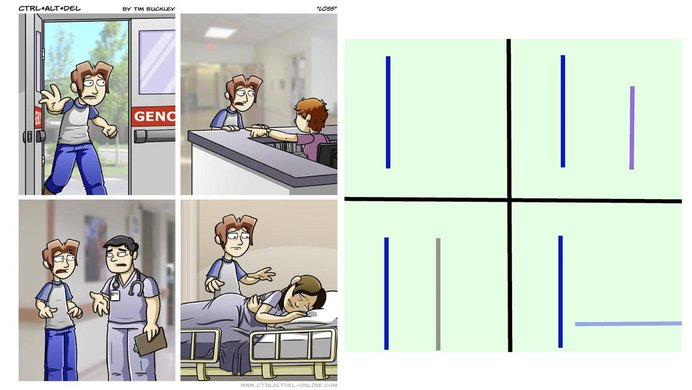
\includegraphics[width=0.8\textwidth]{lossminimal}
\caption{Cómic origianl (izq.), patrón buscado (der.)}
\label{fig:loss}
\end{figure}

\subsection{Datos}

El conjunto de datos consiste de una colección de 1735 imágenes, 1304 para
entrenamiento (con 558 edits) y 431 para verificación (con 185 edits), divididas
en nuestras ya mencionadas dos categorías.

Los memes variados se obtuvieron de la colección personal de memes de los
desarrolladores, obtenidas con el paso del tiempo ya sea descargándolas de
distintos sitios de internet como redes sociales, chats de WhatsApp, Messenger,
etc., mientras que los edits de Loss se descargaron principalmente de la galería
de \textsf{KnowYourMeme.com}\footnote{\url{http://knowyourmeme.com/memes/loss/photos}} y
\textsf{Google Images} (que son miniaturas de distintos sitios, como el subreddit
\textsf{r/lossedits}\footnote{\url{http://reddit.com/r/lossedits}} y
\textsf{KnowYourMeme.com} por lo que puede haber imágenes repetidas en el dataset).

\subsubsection{Preprocesamiento}

El primer paso fue cambiar la resolución de las imágenes para tener un dataset
más uniforme (aunque se reescalarán posteriormente de nuevo pues la red neuronal
necesita entradas de tamaño fijo). Dado que las miniaturas de edits tienen baja
resolución (entre 200 y 300 pixeles de ancho/alto), los memes variados fueron
reescalados para tener una resolución similar (250 pixeles de ancho), después se
dividió el conjunto completo de imágenes en conjuntos de entrenamiento y
verificación de manera aleatoria.

Algunos edits de Loss se basan en el uso de colores, pero en general es la
orientación de los polígonos lo que importa como se ve en la Figura ~\ref{fig:color}.
Para tratar estos casos se construyen modelos que trabajan con imágenes a color
y en escala de grises.

\begin{figure}[h]
\centering
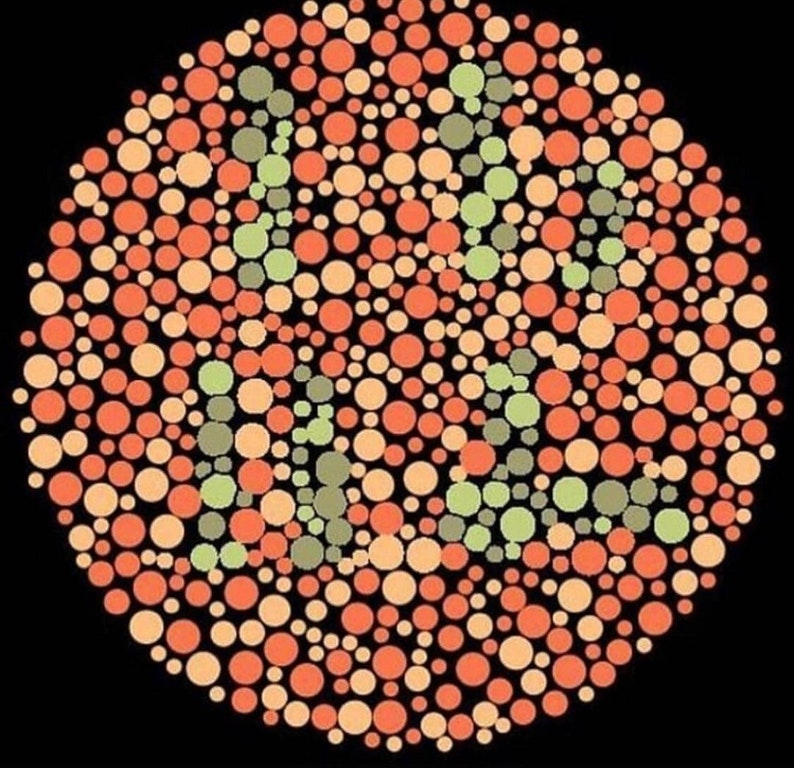
\includegraphics[height=3cm,width=3cm]{loss_color}
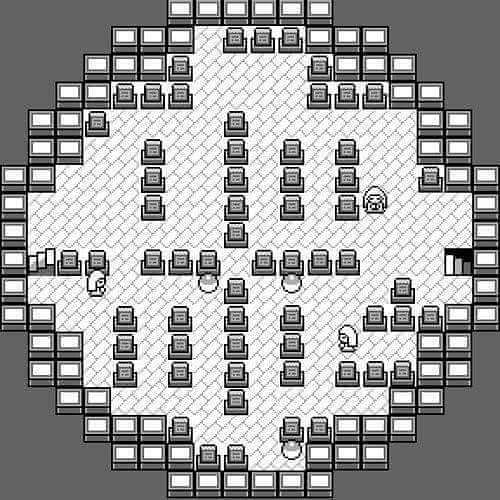
\includegraphics[height=3cm,width=3cm]{pokemon}
\caption{Edit basado en color (izq.) y en orientación (der.)}
\label{fig:color}
\end{figure}

\subsubsection{Problemas con detección de aristas}

Procesar las imágenes para obtener las aristas se consideró una propuesta poco
viable pues se tiene mucho ruido o se pierde información. Usando el modelo
\textsc{Canny} de \textsc{OpenCV} para obtener las aristas presentes en una imagen
nos encontramos con mucho ruido, por ejemplo, si un edit se contruyó con fotografías
con muchos detalles en ellas y objetos innecesarios no fueron desenfocados, las
aristas de dichos objetos se extraen en conjunto con los polígonos que nos
interesan. Si modificamos los umbrales inferior y superior del modelo para filtrar
aristas podemos eliminar aristas de los objetos que nos interesan realmente. Estos
problemas se pueden apreciar en la Figura ~\ref{fig:canny}.

\begin{figure}[h]
\centering
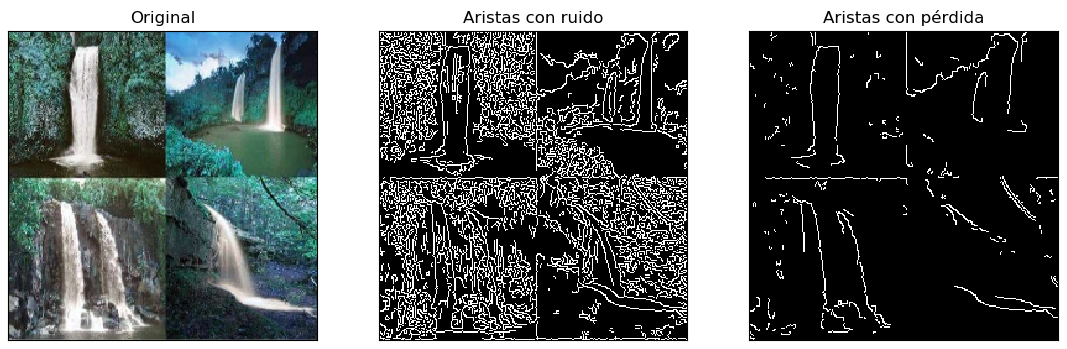
\includegraphics[width=0.8\textwidth]{edges}
\caption{Detección de aristas, algoritmo de Canny.}
\label{fig:canny}
\end{figure}

Además, los umbrales inferior y superior pueden no funcionar en distintas imágenes,
preservando ruido o perdiendo información. La baja resolución de las imágenes
también dificulta este proceso pues los bordes de los contenidos ya no son tan
finos como en la resolución original.

\subsection{Implementación}

La implementación se realizó en el lenguaje de programación \textsc{Python}%
\footnote{Versión 3.6.4, \url{http://www.python.org/downloads/release/python-364/}}.
Para la construcción de la red neuronal convolucional nos apoyamos de los
paquetes \textsc{TensorFlow}\footnote{\url{http://www.tensorflow.org/}} y
\textsc{Keras}\footnote{\url{http://keras.io}}.

\section{Resultados}

\subsection{Pruebas preliminares}

\subsection{Primer intento de clasificación}

\subsection{Segundo intento de clasificación}

\subsection{Observaciones}

\section{Conclusiones}

\begin{thebibliography}{9}
\bibitem{haykin}
Haykin, S. S. (2011).
\textit{Neural networks and learning machines}.
New Dehli: PHI Learning.

\bibitem{wuj}
Wu, J. (2018).
\textit{Convolutional neural networks}.
National Key Lab for Novel Software Technology. Nanjing University, China.
Obtenido de \url{http://cs.nju.edu.cn/wujx/teaching/15_CNN.pdf}.

\bibitem{pooling}
Scherer, D., M\"uller, A., \& Behnke, S. (2010).
\textit{Evaluation of Pooling Operations in Convolutional Architectures for Object Recognition}.
Artificial Neural Networks-ICANN 2010 Lecture Notes in Computer Science, 92-101. DOI:10.1007/978-3-642-15825-4\_10.

\bibitem{lecun}
Lecun, Y., Bottou, L., Bengio, Y., \& Haffner, P. (1998).
\textit{Gradient-Based Learning Applied to Document Recognition}.
Proceedings of the IEEE, 86(11), 2278-2324. DOI:10.1109/5.726791.

\bibitem{adagrad}
Ducji, J., Hazan, E., \& Singer, Y. (2011).
\textit{Adaptive Subgradient Methods for Online Learning and Stochastic Optimization}.
Journal of Machine Learning Research 12, 2121-2159.

\bibitem{adam}
Kingma, D. P. \& Lei Ba, J. (2014).
\textit{Adam: A Method for Stochastic Optimization}.
arXiv:1412.6980. Obtenido de \url{http://arxiv.org/pdf/1412.6980.pdf}.

\end{thebibliography}

\end{document}
